% !TEX root = main.tex
\subsection{第3週目:液体金属pn接合ダイオードの測定}

第2週目に作製した液体金属電極付きpn接合ダイオードの整流特性を評価するため,直流電圧・電流源/モニタを用いてI-V特性を測定する.特に熱処理(アニール)有無による特性の違いを確認する.

\subsubsection*{使用装置}

\begin{itemize}
    \item 直流電圧・電流源/モニタ:ADCMT 6240B
    \item 試料プロービング用ステージ
    \item 液体金属塗布Si基板(熱処理あり/なし)
\end{itemize}

\begin{figure}[H]
    \centering
    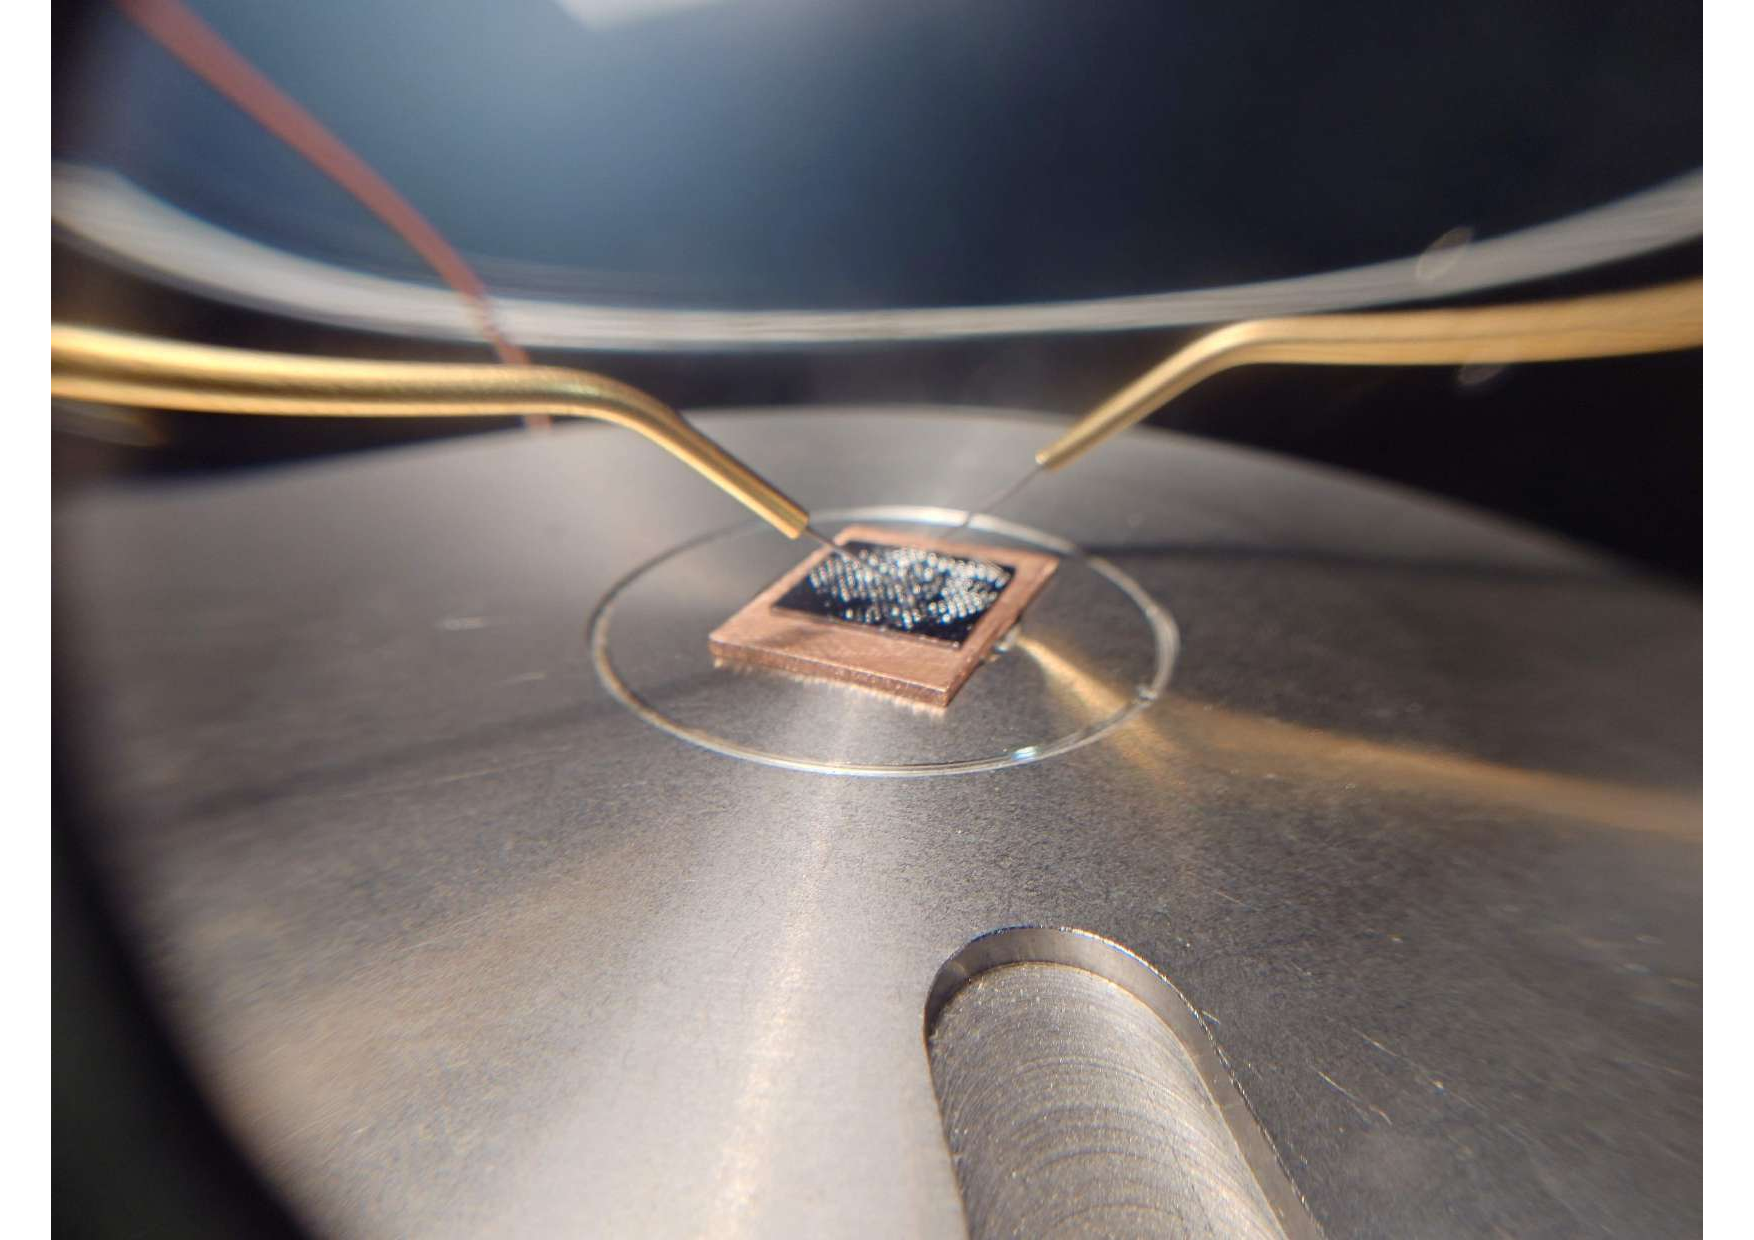
\includegraphics[width=0.6\textwidth]{figure/20250728_133409.pdf}
    \caption{測定中のpn接合ダイオード試料}
    \label{fig:probe_sample}
\end{figure}

\begin{figure}[H]
    \centering
    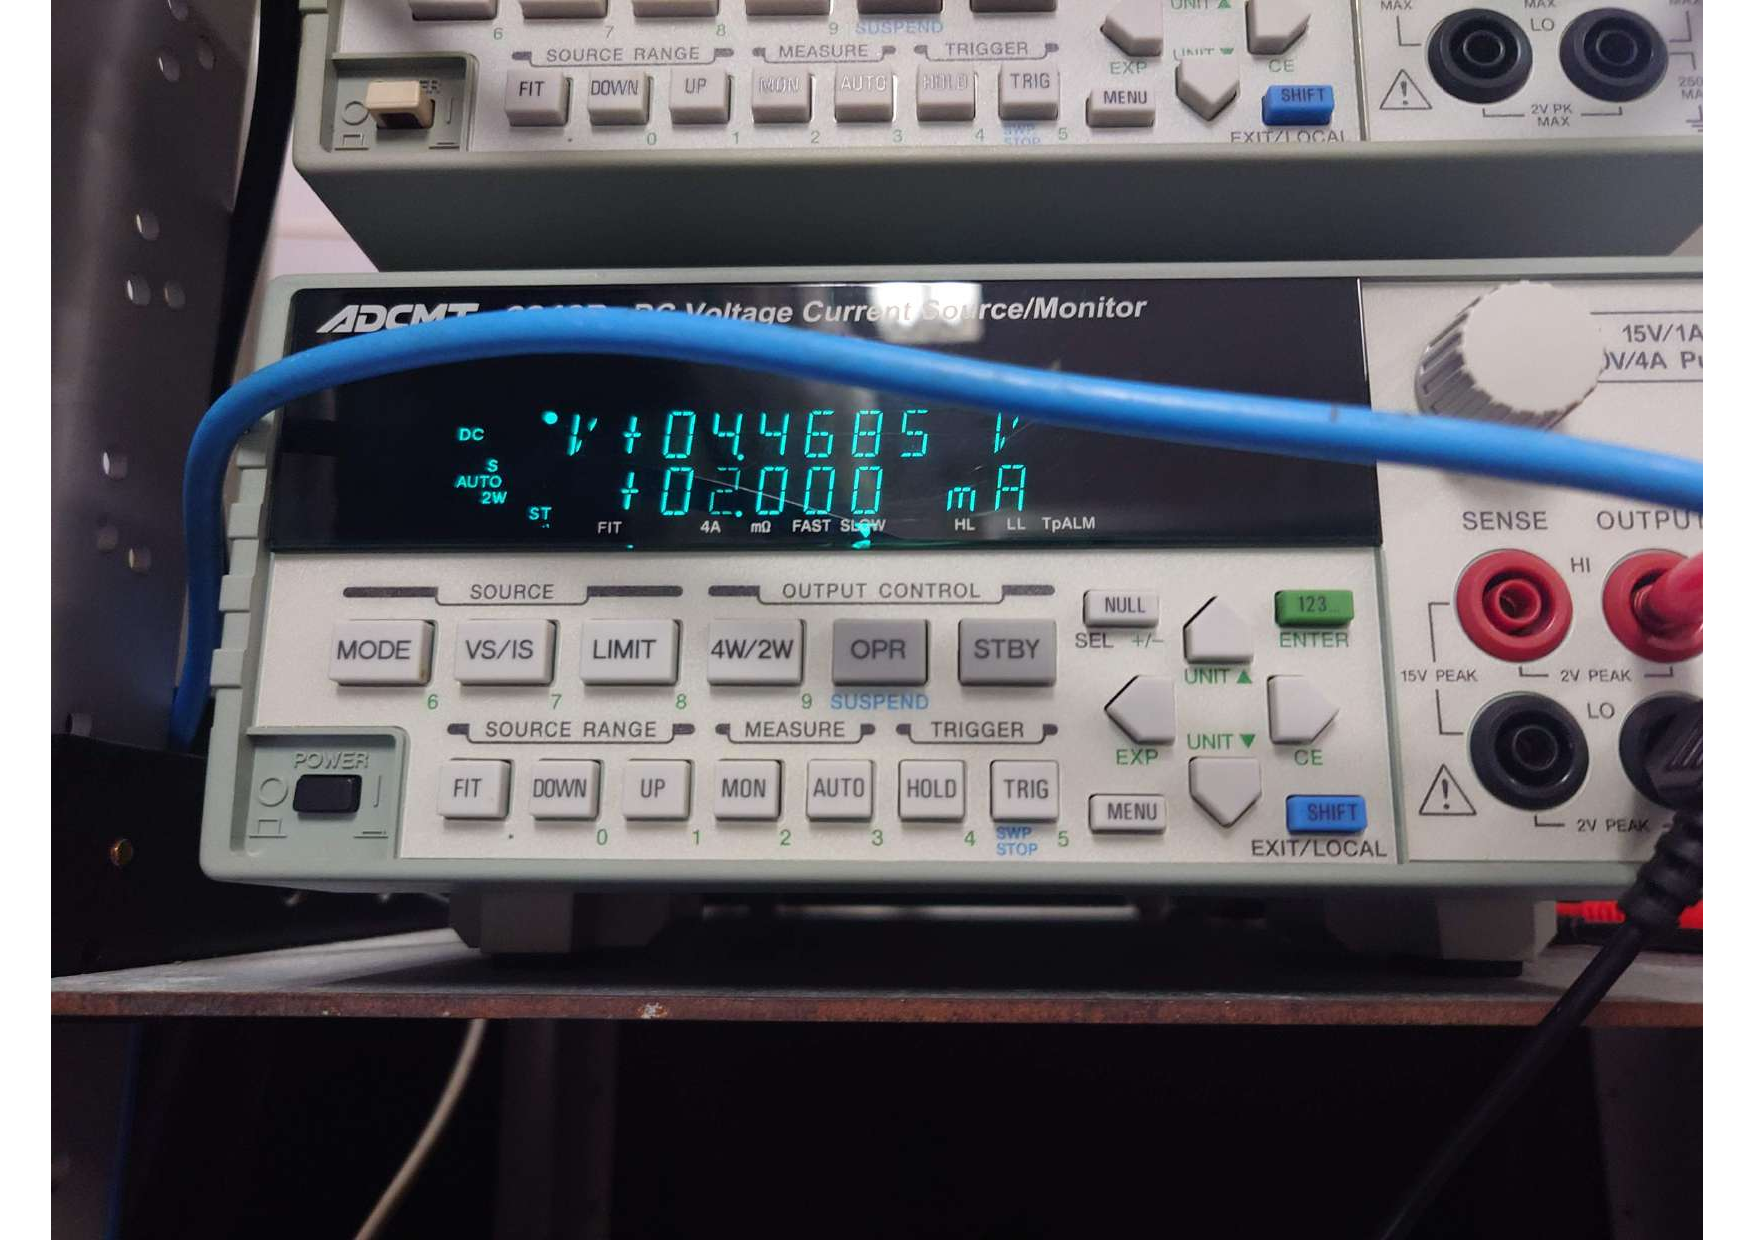
\includegraphics[width=0.6\textwidth]{figure/20250728_131929.pdf}
    \caption{使用した測定装置(ADCMT 6240B)}
    \label{fig:adcmt}
\end{figure}

\subsubsection*{実験手順}

\begin{enumerate}
    \item \textbf{試料設置}:  
    液体金属で電極形成されたpn接合ダイオード試料(熱処理あり・なし)をプロービングステージ上に設置し,プローブを正確に接触させる.

    \item \textbf{装置設定}:  
    ADCMT 6240Bの電圧レンジを設定し,測定対象に適したスイープ範囲(例:\(-1.0~\mathrm{V} \sim 1.0~\mathrm{V}\))を決定.電流測定レンジも適宜自動設定とする.

    \item \textbf{エイジング処理(初期通電)}:  
    液体金属接触部の酸化膜除去と安定化を目的として,測定前に低電圧で連続的に電流を流す.この処理によって酸化膜が破壊され,安定した整流特性が得られるようになる(以下「エイジング」と呼ぶ).

    \item \textbf{I-V測定}:  
    エイジング完了後,DCスイープ電圧を加え,それに対する電流を測定することでI-Vカーブを取得する.熱処理ありとなしの2つの試料で同様の測定を行う.

    \item \textbf{データ記録とプロット}:  
    測定されたデータはCSV形式で記録し,後にプロットして整流特性,対称性,閾値電圧,リーク電流などを比較解析する.
\end{enumerate}

\subsubsection*{測定パラメータ(VIG設定)}
\begin{table}[H]
\centering
\begin{tabular}{|l|l|}
\hline
スイープモード & DC \\ \hline
電圧範囲 & $-3.0 \ \mathrm{V} \sim +2.0 \ \mathrm{V}$ \\ \hline
ステップ電圧 & $0.005 \ \mathrm{V}$ \\ \hline
電流リミット & $0.002 \ \mathrm{A}$ \\ \hline
測定レンジ & AUTO \\ \hline
測定モード & 2端子測定 \\ \hline
ホールド時間 & $10 \ \mathrm{ms}$ \\ \hline
パルス幅 & $25 \ \mathrm{ms}$ \\ \hline
\end{tabular}
\caption{使用した測定条件(VIG設定)}
\end{table}

\subsection{結果及び考察}

\begin{figure}[H]
  \centering
  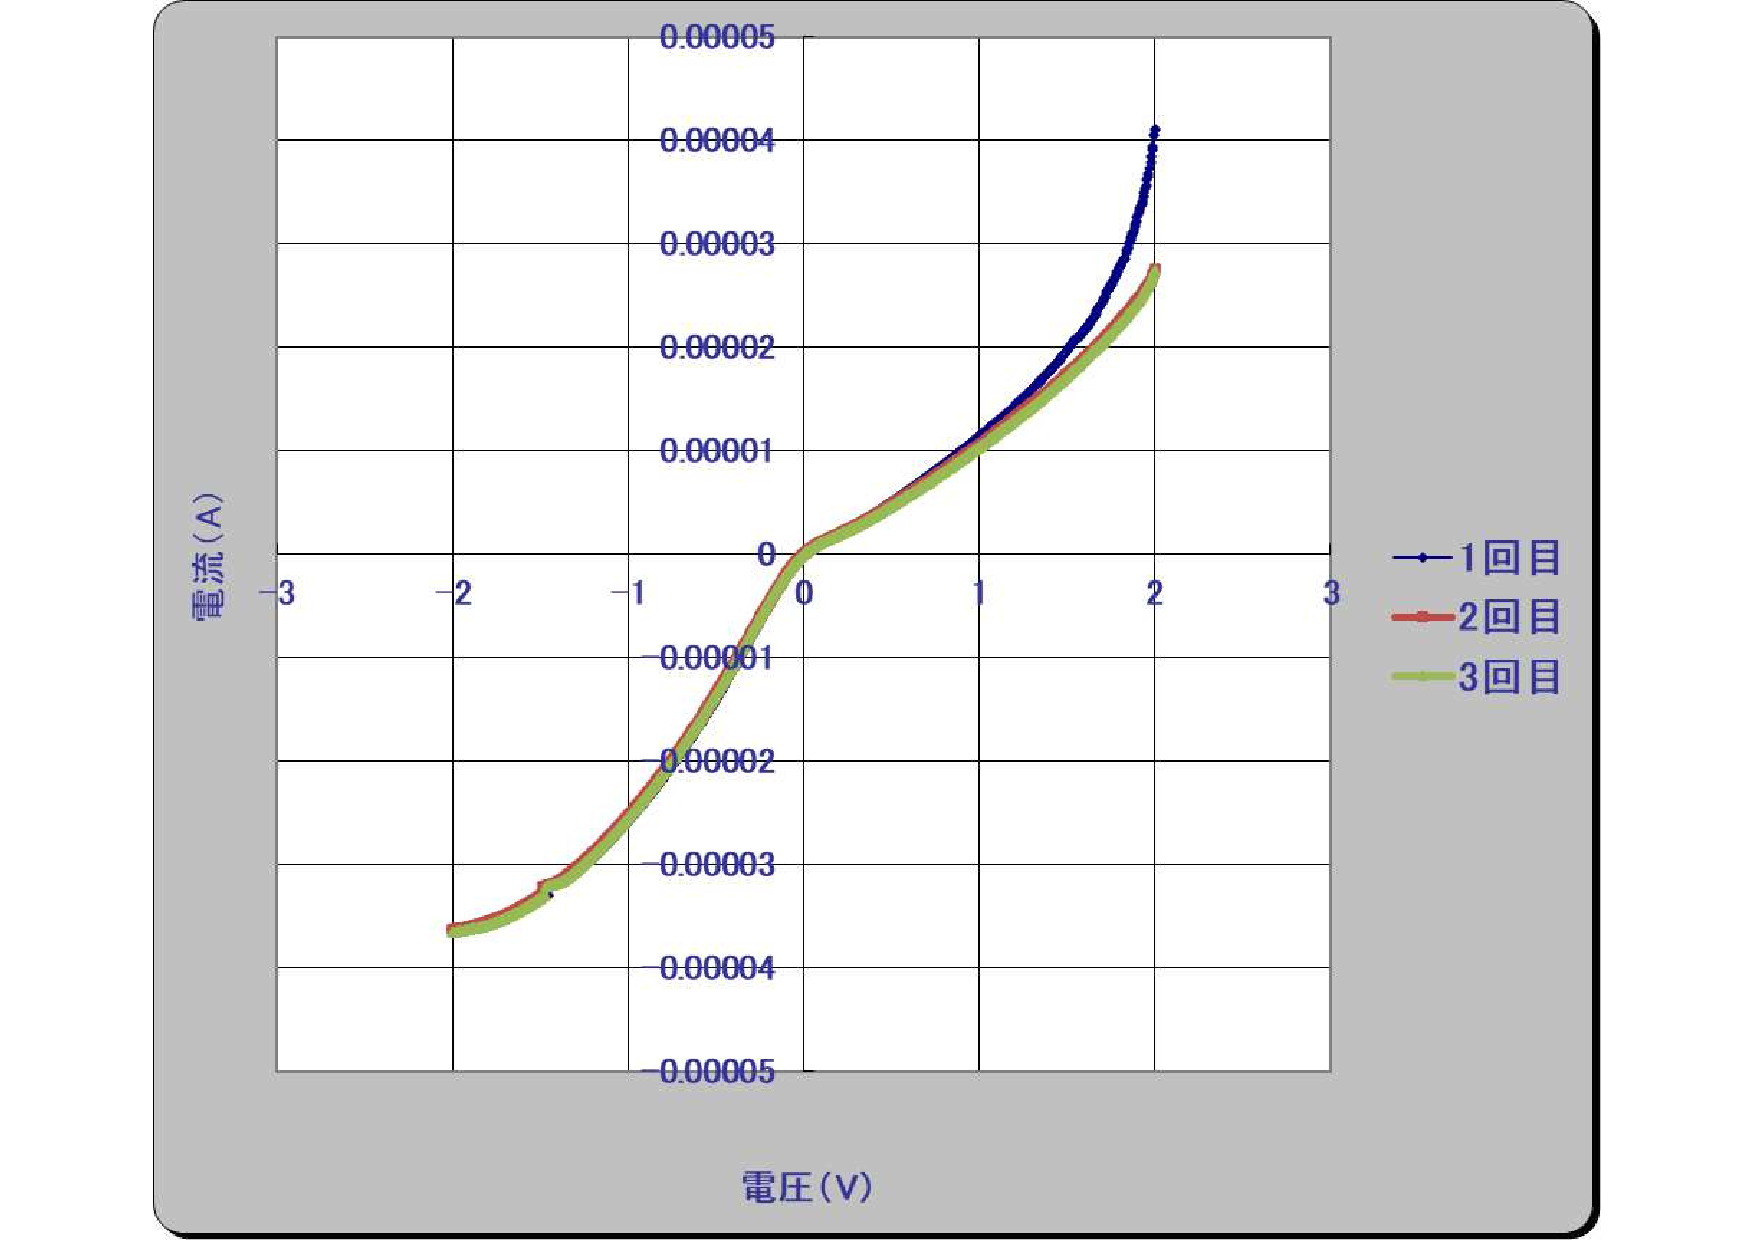
\includegraphics[width=0.65\linewidth]{figure/20250728_1111.pdf} % I-Vグラフ画像
  \caption{I-V測定結果(熱処理あり)}
  \label{fig:iv_heat}
\end{figure}

\begin{figure}[H]
  \centering
  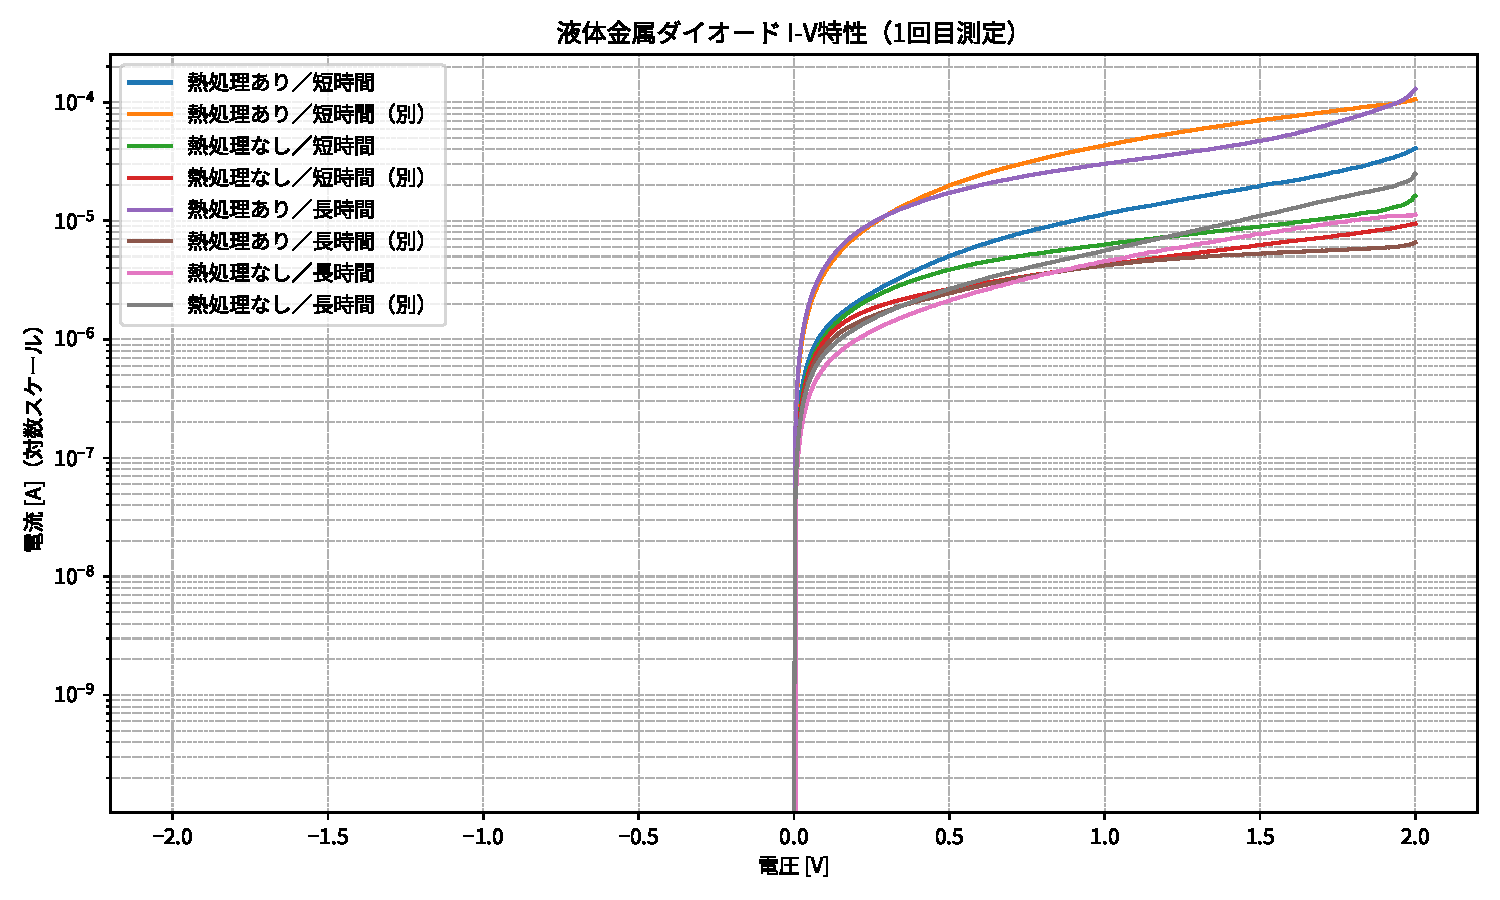
\includegraphics[width=0.75\linewidth]{figure/iv_all_first.pdf}
  \caption{全員分のI-V特性(1回目測定,対数スケール)}
  \label{fig:iv_all_first}
\end{figure}

図\ref{fig:iv_heat}に,熱処理を施した試料におけるI-V測定結果を示す.測定範囲内では,電流値は $10^{-7}~\mathrm{A}$ 以下と極めて微小であり,理想的なダイオードに見られる急峻な立ち上がりは確認できなかった.特に2回目および3回目の測定においては,電流はほぼゼロとなり,ダイオードとしての整流特性は認められなかった.

一方で,1回目の測定では微小ながら電流の増加が観測されたことから,事前に行ったエイジング処理が酸化膜の一部除去に寄与し,短時間的にキャリアの注入が可能になったものと考えられる.

図\ref{fig:iv_all_first}は,全員分の1回目測定結果を対数スケールでまとめたものである.ここでも熱処理を行った試料においては電流値が顕著に小さく,整流特性が見られなかった一方,熱処理を行っていない試料では,なだらかではあるが順方向の電流増加が確認された.この結果は,熱処理によってSi基板および液体金属電極表面に形成された酸化膜が,キャリア注入の障壁として機能した可能性を強く示唆している.

また,液体金属の塗布厚さや基板との接触状態が試料ごとに異なることも,I-V特性にばらつきが生じた一因と考えられる.とりわけ液体金属が基板の側面に回り込む現象や,表面に酸化物が残存することにより,意図しない電流経路や高い接触抵抗が発生した可能性も否定できない.

今後の改善点としては,熱処理条件の最適化だけでなく,酸化膜の除去プロセス(例:化学洗浄やプラズマ処理)の導入,および電極形成プロセスの均一性向上が挙げられる.これにより,液体金属を用いたダイオードの再現性および整流性能の向上が期待される.
